\section{Scaling Laws of Learning from Real World Environments}
\label{sec:emerging-scaling}

Pretraining scaling laws classically model language-model loss as a power-law
function of training scale, including the amount of pretraining
data~\citep{kaplan2020scaling,hoffmann2022training}. By contrast, benchmark
performance is a task-level readout of model capability, shaped by the
difficulty thresholds induced by tasks, examples, and scoring criteria. Prior
work has found that it is well described under pretraining scale-up by a
log-sigmoid curve
~\citep{dubey2024llama3,bhagia2024taskscaling,owen2024predictable,
ruan2024observational}.

Beyond learning from human-collected training data, modern agents such as
GPT-5.5 and Claude Opus 4.8 can continue to learn from their environments after
deployment. On a
task, they can acquire new information through interaction and improve their
performance over time. Yet it remains
unclear whether this form of learning obeys any similarly simple scaling law.
\benchmark{} provides 134 diverse real world tasks with executable
environments, informative feedback, and at least 12-hour interaction windows, allowing
us to study how agents improve through interaction with their environments.
Analyzing five frontier agents over roughly \textbf{38,000 hours of environment
interaction} across 134 diverse real world tasks, we find that \textbf{a
log-sigmoid curve fits environment learning performance precisely}. Thus,
learning from the environment and learning from pretraining data induce the
same mathematical scaling form.

\subsection{From Task Trajectories to Predictable Scaling Curves}
\label{sec:environment-learning-data}

\underline{\textit{Experimental setting.}} We evaluate 134 \benchmark{} tasks
with five frontier models: Claude Opus 4.8~\cite{anthropic2026claudeopus48systemcard}, GPT-5.5~\cite{openai2026gpt55systemcard}, GPT-5.4~\cite{openai2026gpt54thinkingsystemcard}, GLM-5.1~\cite{zai2026glm51,glm5team2026glm5report}, and
DeepSeek-V4-Pro (preview)~\cite{deepseekai2026deepseekv4}. For each task--model pair, we run three independent 12-hour trials and record the
full submission trajectory. GPT models are run with Codex using a 256k compact
window, while GLM-5.1 and DeepSeek-V4-Pro are run with Claude Code using 200k
compact windows. Claude Opus 4.8 is primarily run with a 1M Claude Code compact
window; we additionally include a 200k versus 1M Opus ablation in
Section~\ref{sec:context-length-analysis}.

\underline{\textit{Per-task trajectory diversity.}} Figure~\ref{fig:environment-data-curves-copy} shows per-task learning curves
for 18 representative tasks, illustrating how different models improve on the
same task over time. The full set of per-task curves is provided in
Appendix~\ref{sec:all-curves} for all 134 tasks. The tasks span diverse domains
and exhibit heterogeneous learning dynamics, with trajectories ranging from
smooth incremental gains to long plateaus, abrupt breakthroughs, and irregular
regressions.

\underline{\textit{Aggregate curves reveal a common structure.}} Although these individual curves are heterogeneous across both tasks and
models, their cross-task averages are unexpectedly smooth and share a common
structure. Motivated by prior log-sigmoid fits of benchmark performance under
pretraining scale-up, we fit the averaged environment learning curves with the
following three-parameter log-sigmoid model:
\begin{equation}
    S(t)
    =
    \frac{S_{\max}}{1 + (t_{\mathrm{mid}} / t)^\beta},
    \label{eq:log-sigmoid-learning}
\end{equation}
where $t$ is elapsed interaction time and $S(t)$ is best-so-far
performance. The fitted parameters serve as empirical descriptors of the
aggregate learning curve: $S_{\max}$ is the attainable score ceiling,
$t_{\mathrm{mid}}$ is the interaction time at which the curve reaches half of
that ceiling, and $\beta$ controls how sharply progress concentrates in log
time. Thus a smaller $t_{\mathrm{mid}}$ means the model reaches the bulk of its
attainable score sooner, while a larger $\beta$ corresponds to a steeper
learning transition. Section~\ref{sec:log-sigmoid-fit} shows that this simple
functional form fits the empirical learning curves surprisingly well.

\begin{figure}[!t]
\centering
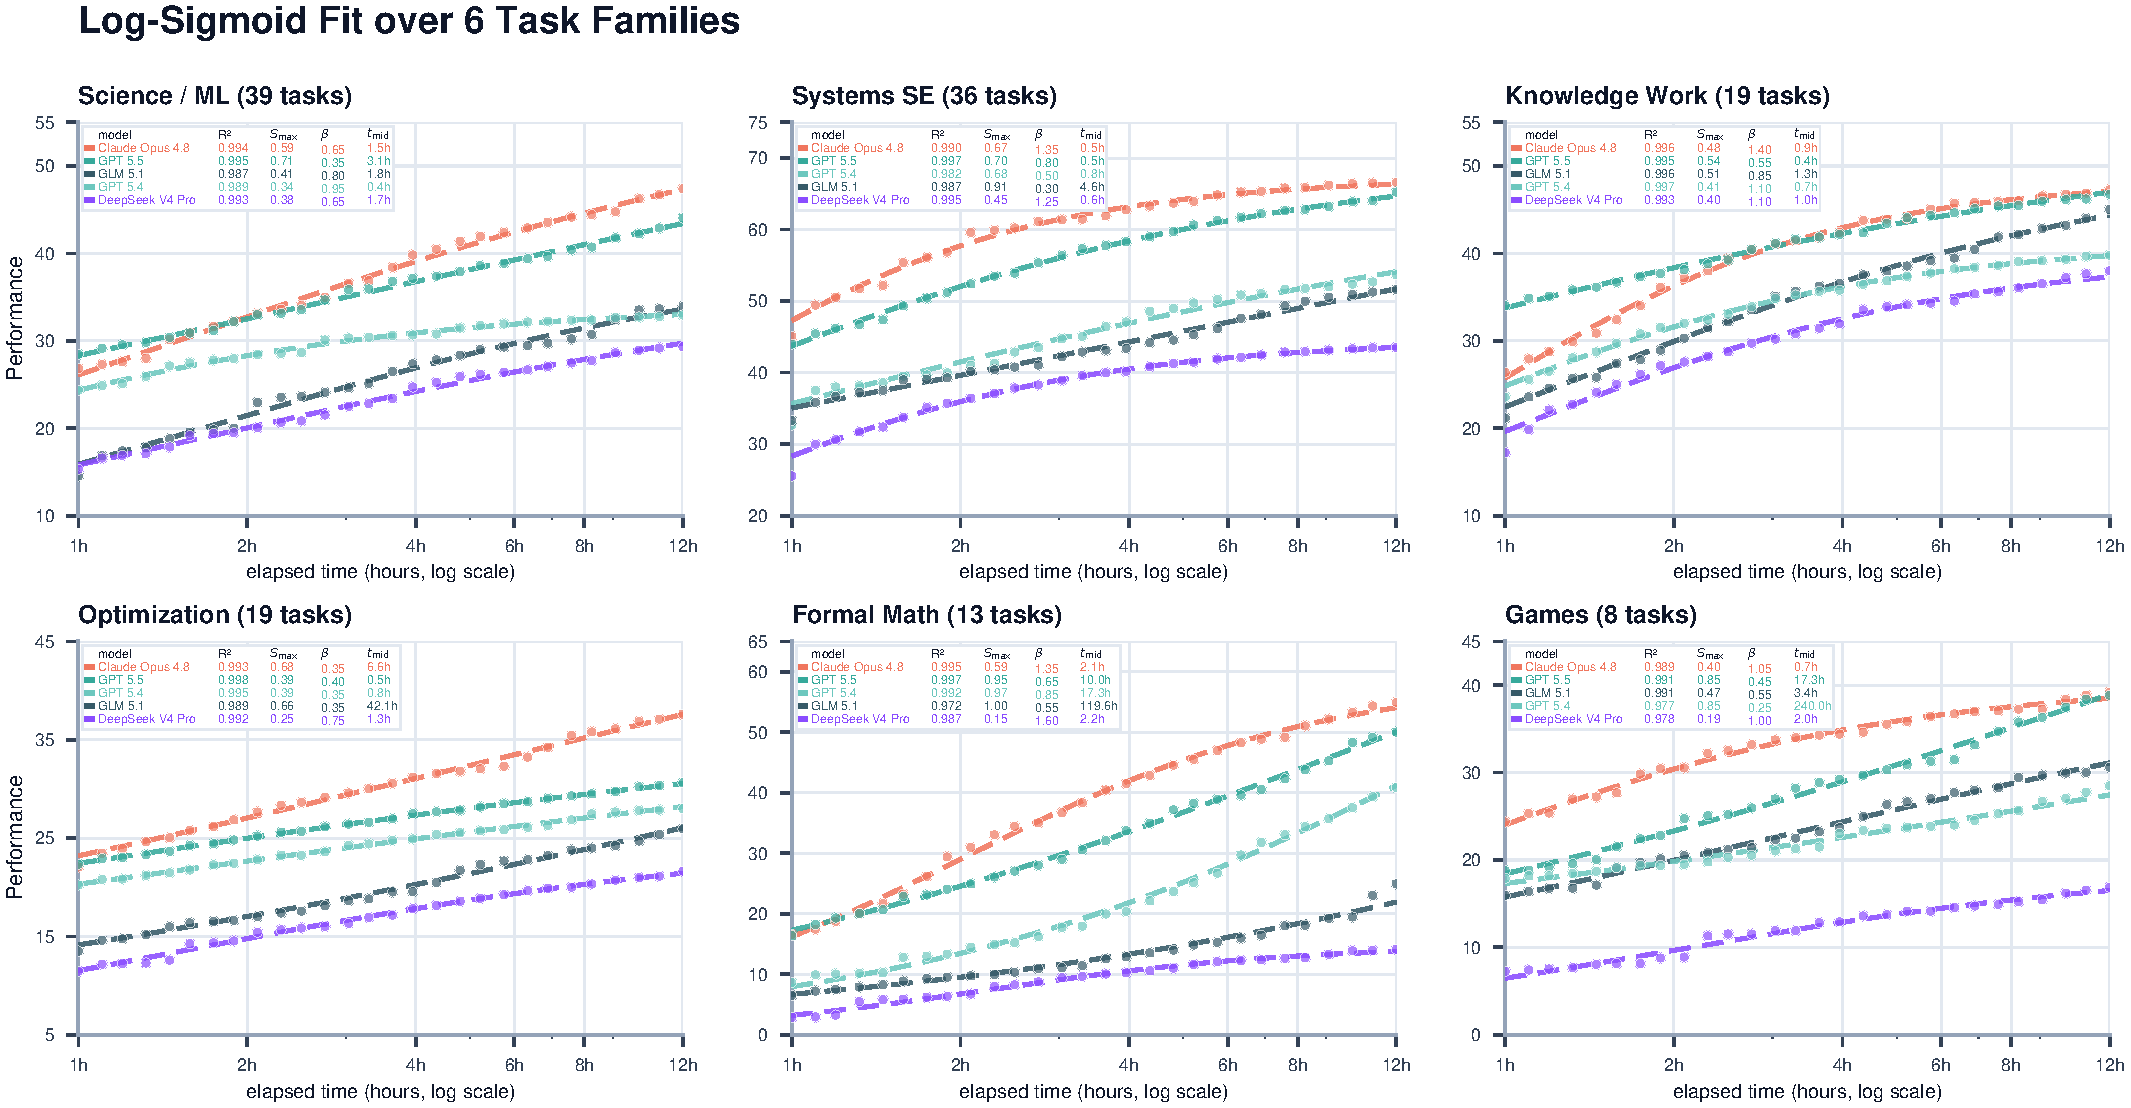
\includegraphics[width=\linewidth]{figures/logtime_sigmoid_domains_1h_12h.pdf}
\caption[Task-family-level log-sigmoid fits across the six \benchmark{} task families.]{
Task-family-level log-sigmoid fits across the six \benchmark{} task families.
Despite large differences in task type and scoring function, the same
log-time sigmoidal form fits the average trajectory in each task family well.\protect\footnotemark}
\label{fig:logtime-sigmoid-domains}
\end{figure}
\footnotetext{Fit precision improves as the number of fitted tasks increases; see
Figure~\ref{fig:log-sigmoid-rmse-task-count}.}

\begin{figure}[!t]
\centering
\begin{minipage}[t]{0.64\linewidth}
\centering
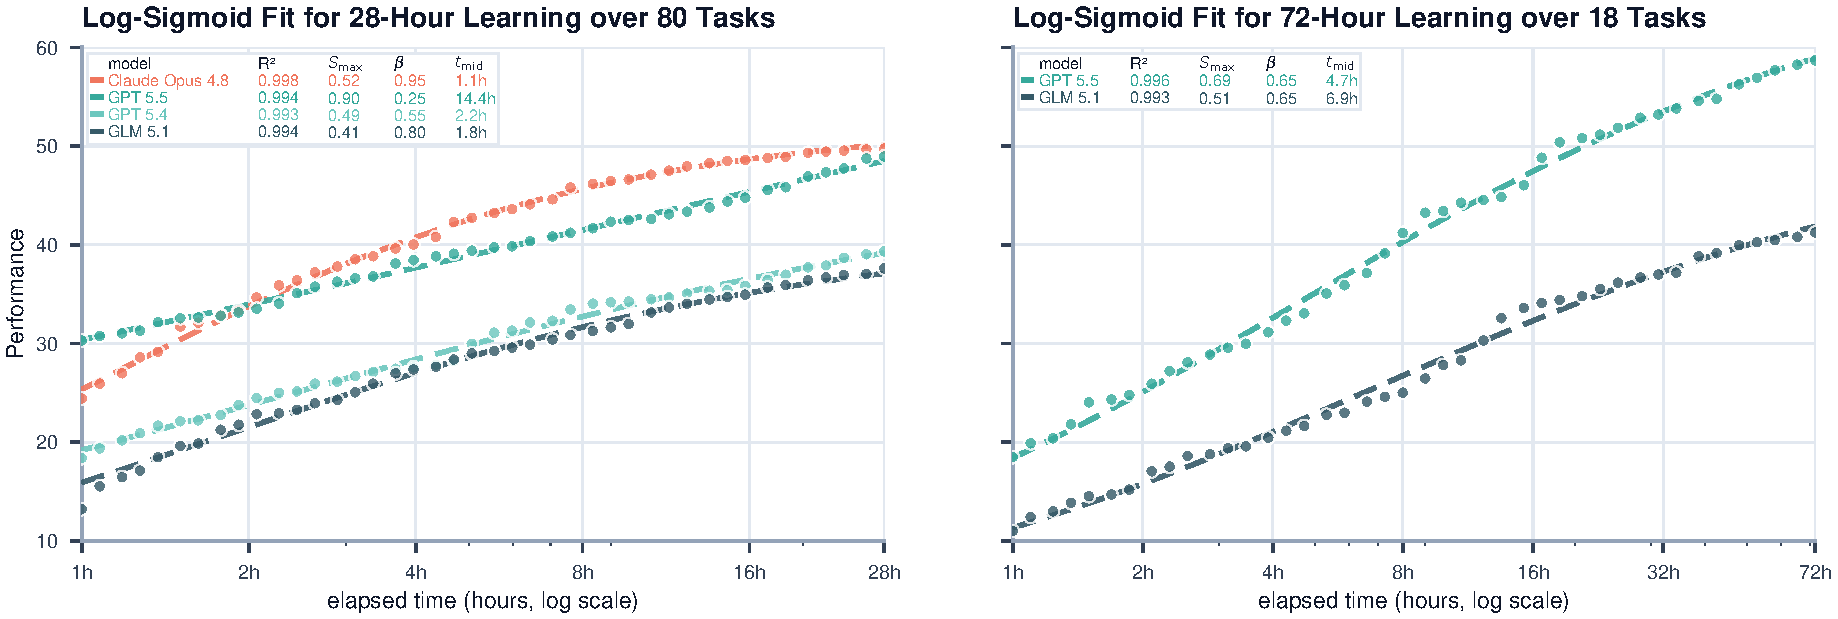
\includegraphics[width=\linewidth]{figures/logtime_sigmoid_long_horizon_28h_72h.pdf}
\caption{Long-horizon log-sigmoid fits beyond the main 12-hour benchmark window.
The left panel fits 28-hour trajectories averaged over 80 tasks; the right panel fits
72-hour trajectories averaged over 18 tasks. All fitted curves remain highly precise,
with $R^2 \geq 0.993$.}
\label{fig:long-horizon-sigmoid-fits}
\end{minipage}
\hfill
\begin{minipage}[t]{0.32\linewidth}
\centering
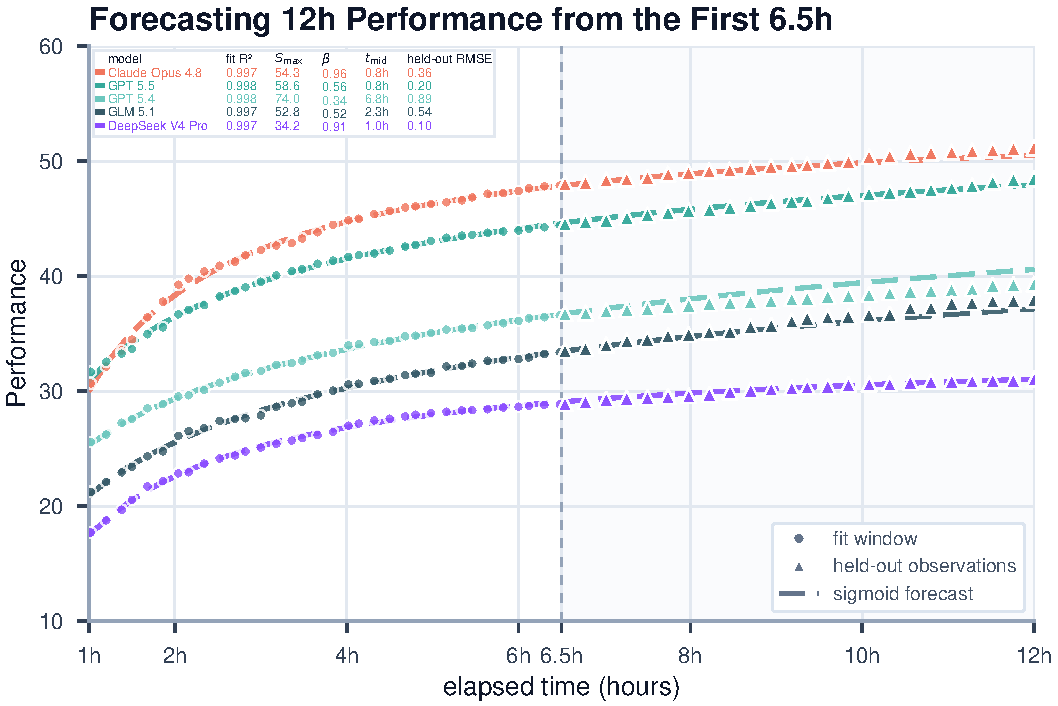
\includegraphics[width=\linewidth]{figures/logtime_sigmoid_forecast_1h_6p5h_to_12h.pdf}
\caption[Forecasting 12-hour performance from the first 6.5 hours.]{
Forecasting 12-hour performance from the first 6.5 hours. Log-sigmoid
fits on this early window accurately predict the held-out remainder for all five
models.\protect\footnotemark}
\label{fig:sigmoid-forecast-6p5h}
\end{minipage}
\end{figure}
\footnotetext{GPT-5.4 service availability dropped in the latter half of the
experiment, which may partly explain its forecast deviation; see
Appendix~\ref{sec:gpt54-serving-stability}.}

\subsection{Log-Sigmoid Curves Fit Environment Learning with Remarkable Precision}
\label{sec:log-sigmoid-fit}

We find that the log-sigmoid fit is precise and robust across every setting we tested:

\begin{itemize}
    \item \textbf{Log-sigmoid curves precisely fit the 134-task average for all
    five models.}
    As shown in Figure~\ref{fig:logtime-sigmoid-all-tasks}, after averaging
    over all 134 tasks, the fitted log-sigmoid curve closely tracks each
    model's 12-hour learning trajectory. The fit is uniformly tight across all
    five models, with $R^2 \geq 0.997$ in every case.

    \item \textbf{The same log-sigmoid form persists across heterogeneous task families.}
    Figure~\ref{fig:logtime-sigmoid-domains} repeats the fit separately across
    the six capability families in \benchmark{}. These families require different knowledge,
    exercise different capabilities, and produce visibly different aggregate
    learning curves. Yet each family is still well described by the same
    log-sigmoid form, including smaller families where fewer tasks make the
    averaged trajectories noisier.

    \item \textbf{The fit remains precise under substantially longer
    interaction horizons.}
    Figure~\ref{fig:long-horizon-sigmoid-fits} extends the analysis beyond the
    main 12-hour window to 28-hour and 72-hour interaction horizons. Due to
    resource limits, the 28-hour fit covers 80 tasks and four models, while
    the 72-hour fit covers 18 tasks and two models. The same log-sigmoid
    structure remains stable across both longer settings, with every fitted
    curve reaching $R^2 \geq 0.993$.

    \item \textbf{The log-sigmoid law exhibits predictive power.}
    Figure~\ref{fig:sigmoid-forecast-6p5h} tests this by fitting each
    12-hour aggregate curve using only the first 6.5 hours, then evaluates the forecast on
    held-out observations from 6.5 to 12 hours. The extrapolated curves remain
    close to the later observed trajectories across all five models, with
    $R^2 \geq 0.997$ and RMSE below 1.0 performance point in every case.

\end{itemize}

These precise fits raise two questions: is the log-sigmoid genuinely the right curve, or would any S-shape do, and where does so clean a law come from?

\underline{\textit{Log-sigmoid fits best among common S-curves.}}
Many saturating growth processes are S-shaped~\citep{wikipedia_scurve}. We therefore
compare the log-sigmoid against other common S-curves, each viewing an
S-shaped learning curve as a cumulative distribution over a time coordinate:
log-probit~\citep{bliss1934method}, log-Gompertz~\citep{gompertz1825nature}, and
a Weibull CDF~\citep{weibull1951statistical} on raw time, together with a
two-parameter log-linear baseline; for the log-time families the independent
variable is $x=\ln t$. We fit every family on the 12h, 28h, and 72h full windows
and pool the error. As Table~\ref{tab:scurve-family-comparison} shows, the log-sigmoid
family attains the lowest RMSE, while the log-linear baseline is substantially worse. The empirical
signal is thus robustly sigmoidal rather than tied to a single link function,
and is not explained by mere linear improvement in $\ln t$. Appendix~\ref{sec:scurve-mechanistic-reading}
discusses why we nevertheless prefer the log-sigmoid on mechanistic grounds.

\begin{figure}[!t]
\centering
\begin{minipage}[t]{0.57\textwidth}
\vspace{0pt}
\small
\renewcommand{\arraystretch}{1.42}
\setlength{\tabcolsep}{4pt}
\resizebox{\ifdim\width>\linewidth\linewidth\else\width\fi}{!}{%
\begin{tabular}{@{}>{\raggedright\arraybackslash}p{0.22\linewidth}
                >{\raggedright\arraybackslash}p{0.58\linewidth}
                r@{}}
\BenchTopRule
Family & Functional form & RMSE \\
\BenchMidRule
\textbf{Log-Sigmoid} &
$\displaystyle S(t)=\frac{S_{\max}}{1+(t_{\mathrm{mid}}/t)^{\beta}}$ &
\textbf{0.390} \\
\addlinespace[2pt]
Log-Probit &
$\displaystyle S(t)=S_{\max}\,\Phi\!\left(\frac{\ln t-\mu}{\sigma}\right)$ &
0.398 \\
\addlinespace[2pt]
Log-Gompertz &
$\displaystyle S(t)=S_{\max}\exp\!\left[-\exp\{-c(\ln t-x_0)\}\right]$ &
0.402 \\
\addlinespace[2pt]
Weibull CDF &
$\displaystyle S(t)=S_{\max}\left(1-\exp\{-(t/\lambda)^\beta\}\right)$ &
0.404 \\
\addlinespace[2pt]
Log-Linear &
$\displaystyle S(t)=a+b\ln t$ &
0.717 \\
\BenchBottomRule
\end{tabular}%
}
\captionof{table}{Full-window fit error for three-parameter S-curve families and a
two-parameter log-linear baseline. RMSE is measured in \underline{performance
points} on the 0--100 score scale; lower is better.}
\label{tab:scurve-family-comparison}
\end{minipage}
\hfill
\begin{minipage}[t]{0.39\textwidth}
\vspace{0pt}
\centering
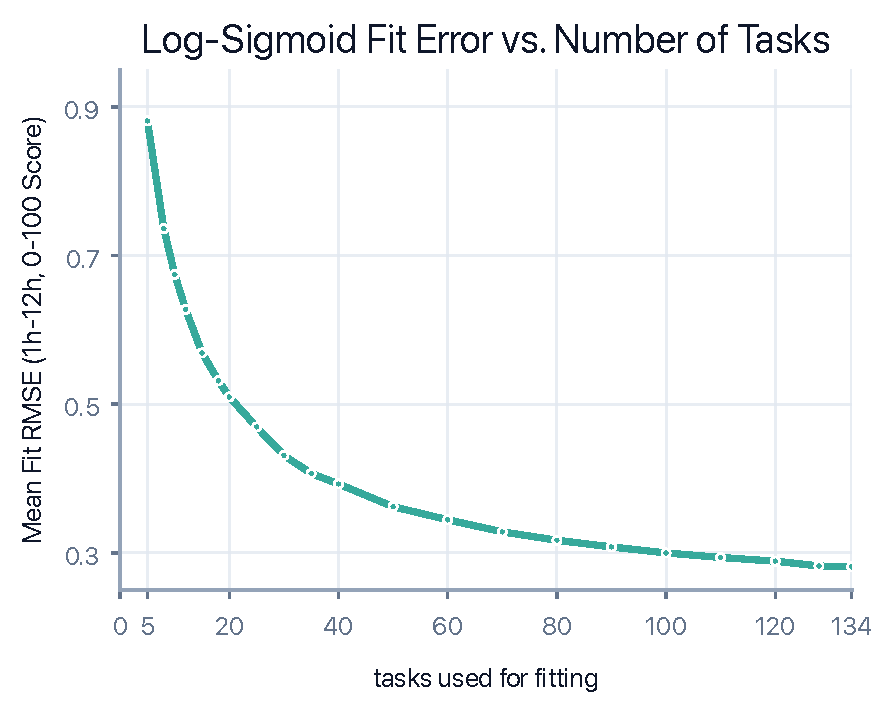
\includegraphics[width=\linewidth]{figures/fig_12h_log_sigmoid_rmse_1_to_134_tasks_repo_style.pdf}
\captionof{figure}{Log-sigmoid fit error decreases as more tasks are averaged.}
\label{fig:log-sigmoid-rmse-task-count}
\end{minipage}
\end{figure}

\underline{\textit{The law emerges from a population of tasks.}}
A single task's trajectory is noisy and idiosyncratic, yet
Figure~\ref{fig:log-sigmoid-rmse-task-count} shows that the log-sigmoid fit
becomes steadily more precise as we average over more tasks: the residual error
falls monotonically as tasks accumulate, from $1$ task to all $134$. The clean
scaling law is therefore an \emph{emergent, population-level} regularity, sharp
only across many diverse tasks rather than within any one of them. 

\FloatBarrier

\subsection{A Theory of the Log-Sigmoid Law}
\label{sec:why-log-sigmoid}

The empirical fits show a robust log-sigmoid shape, but do not by themselves explain why this form should appear. We propose a theoretical model: environment learning is a frontier expansion process on the underlying task graphs. In this view, each task is modeled by a latent graph of score units, the already-unlocked units exert influence on the locked neighbors to unlock them, and progress occurs when the frontier between unlocked and locked score nodes advances. Appendix~\ref{sec:theory} gives the full derivation; here we summarize the mechanism. Throughout the section, we use 
\[
u = \log t - \log t_{\mathrm{mid}}
\] 
as a change of coordinate of the time axis.

\underline{\textit{Environment learning is a frontier expansion process.}}
For a single task, let us consider the task score is composed of many score units, representing nodes \(i\) on the task graph \(G\) with score \(w_i\) and normalized score weights \(\mu_i = w_i / \sum_i w_i\). Let \(n_i(u)\in\{0,1\}\) indicate whether unit \(i\) has been unlocked at time \(u\), the normalized score obtained is
\[
    x(u)=\sum_i \mu_i n_i(u).
\]
On the task graph \(G\), an edge weight \(K_{ij}\ge0\) measures how much an unlocked source unit \(j\) helps unlock a target unit \(i\). Thus a locked unit \(i\) receives an influence field
\[
    h_i(u)=\sum_j K_{ij}n_j(u).
\]
If locked units unlock randomly at an expected rate proportional to this field, then conditioned on the current state,
\begin{equation}
    \label{eq:frontier-expansion-naive}
    \frac{\mathrm d}{\mathrm du}\mathbb E[x(u)\mid n(u)]= \eta \sum_{i\in L(u)}\sum_{j\in U(u)}\mu_iK_{ij}.
\end{equation}
The expected score-growth rate is therefore exactly the weighted frontier cut from unlocked units \(U(u)\) to locked units \(L(u)\).

\underline{\textit{Frontier process moves at a speed proportional to \(x(1-x)\).}}
The exact frontier cut still depends on the task graph structure. The mean-field approximation is to assume that, at the aggregate level, every macroscopic unlocked--locked cut has approximately product-measure influence:
\[
    \sum_{i\in L}\sum_{j\in U}\mu_iK_{ij}
    \approx
    \kappa \mu(L)\mu(U).
\]
where \(\mu(A) = \sum_{i\in A} \mu_i\) for any set \(A \subseteq G\). This, along with \eqref{eq:frontier-expansion-naive}, gives
\begin{equation}
    \label{eq:logistic-dynamics-naive}
    \frac{\mathrm dx}{\mathrm du} = \beta x(1-x),\qquad \beta=\eta\kappa.
\end{equation}
The two factors have direct interpretations: unlocked score mass supplies reusable capability, while locked score mass measures the remaining opportunity for improvement. Appendix~\ref{subsec:single-task-frontier} formalizes this approximation using a weighted cut-mixing condition, which is weaker than assuming that all edge weights are individually equal.

\underline{\textit{The effective time coordinate is logarithmic.}}
The frontier equation is written in an effective task-graph coordinate \(u\). A natural reason for \(u\) to be approximately \(\log t\) is self-similar graph structure\footnote{This resembles scale-free dynamics in physical complex systems, such as self-organized criticality and critical phenomena, where behavior is not governed by a single characteristic scale~\citep{bak1987self,newman2005power}.}. If each additive increase in task difficulty exposes a multiplicatively larger amount of relevant graph structure, then search volume needed to traverse the graph grows exponentially with difficulty scale. If the search effort is approximately constant across time horizon, then the difficulty scale reached by time \(t\) grows as 
\[
    u \sim \log t
\]
Substituting this coordinate into the frontier equation~\eqref{eq:logistic-dynamics-naive} gives
\begin{equation}
    \label{eq:log-sigmoid-curve-naive}
    \frac{\mathrm dx}{\mathrm d\log t} = \beta x(1-x).
\end{equation}

\underline{\textit{Solving the frontier equation.}}
Separating variables in \eqref{eq:log-sigmoid-curve-naive} gives
\[
    \log\frac{x(t)}{1-x(t)}
    =
    \beta\log\frac{t}{t_{\mathrm{mid}}},
\]
where \(t_{\mathrm{mid}}\) is chosen so that \(x(t_{\mathrm{mid}})=1/2\). Hence
\[
    x(t) = \frac{1}{1+(t_{\mathrm{mid}}/t)^\beta}, \quad \implies \quad S(t) = \frac{S_{\max}}{1+(t_{\mathrm{mid}}/t)^\beta}.
\]

\underline{\textit{Benchmark average is smoother than individual tasks.}}
The argument above describes the limiting frontier drift. It does not imply that every finite task should visibly follow a smooth sigmoid. A task with a small number of score units can have long plateaus and sudden jumps. The empirical scaling law is instead a statement about the task-aggregate curve. If many independently evaluated tasks each follow approximate frontier dynamics, then averaging removes finite-task jaggedness. The aggregate becomes a single log-sigmoid when residual task midpoints and task speeds concentrate:
\[
    x_M(u)
    =
    \frac1M\sum_{b=1}^M x_b(u)
    \approx
    \frac1M\sum_{b=1}^M
    \frac{1}{1+e^{-\beta_b(u-\delta_b)}}
    \stackrel{P}{\longrightarrow}
    \frac{1}{1+e^{-\beta u}}.
\]
Appendix~\ref{subsec:aggregate-frontier-limit} makes this statement precise under assumptions of blockwise cut-mixing, vanishing average jump noise, midpoint alignment, and speed concentration.

\underline{\textit{Interpretation of the fitted parameters.}}
The fitted rate \(\beta\) has a natural interpretation as an effective frontier-propagation speed in log time. A larger \(\beta\) means that score unlocks over a narrower range of interaction scales, producing a steeper transition from low to high performance. A smaller \(\beta\) means that progress is spread over more multiplicative time, producing a more gradual learning curve. The fitted ceiling \(S_{\max}\) should be interpreted as the attainable score support over the fitted regime, not necessarily as an absolute upper bound on performance.

\underline{\textit{Applicability and limitations.}}
The log-sigmoid law is not expected to hold for every environment-learning process. It can fail when task graphs contain strong bottlenecks, dispersed task midpoints, heterogeneous frontier speeds, or non-scale-free graph structures. These failure modes clarify the scope of the theory: the log-sigmoid is most natural when progress behaves like a sufficiently mixed frontier expansion process on an approximately fractal structured graph. In this sense, learning from environments tests whether an agent can convert diverse feedback into reusable structure that accelerates subsequent discovery. We view this as central to why environment learning is worth measuring and scaling.


\begin{figure}[!t]
\centering
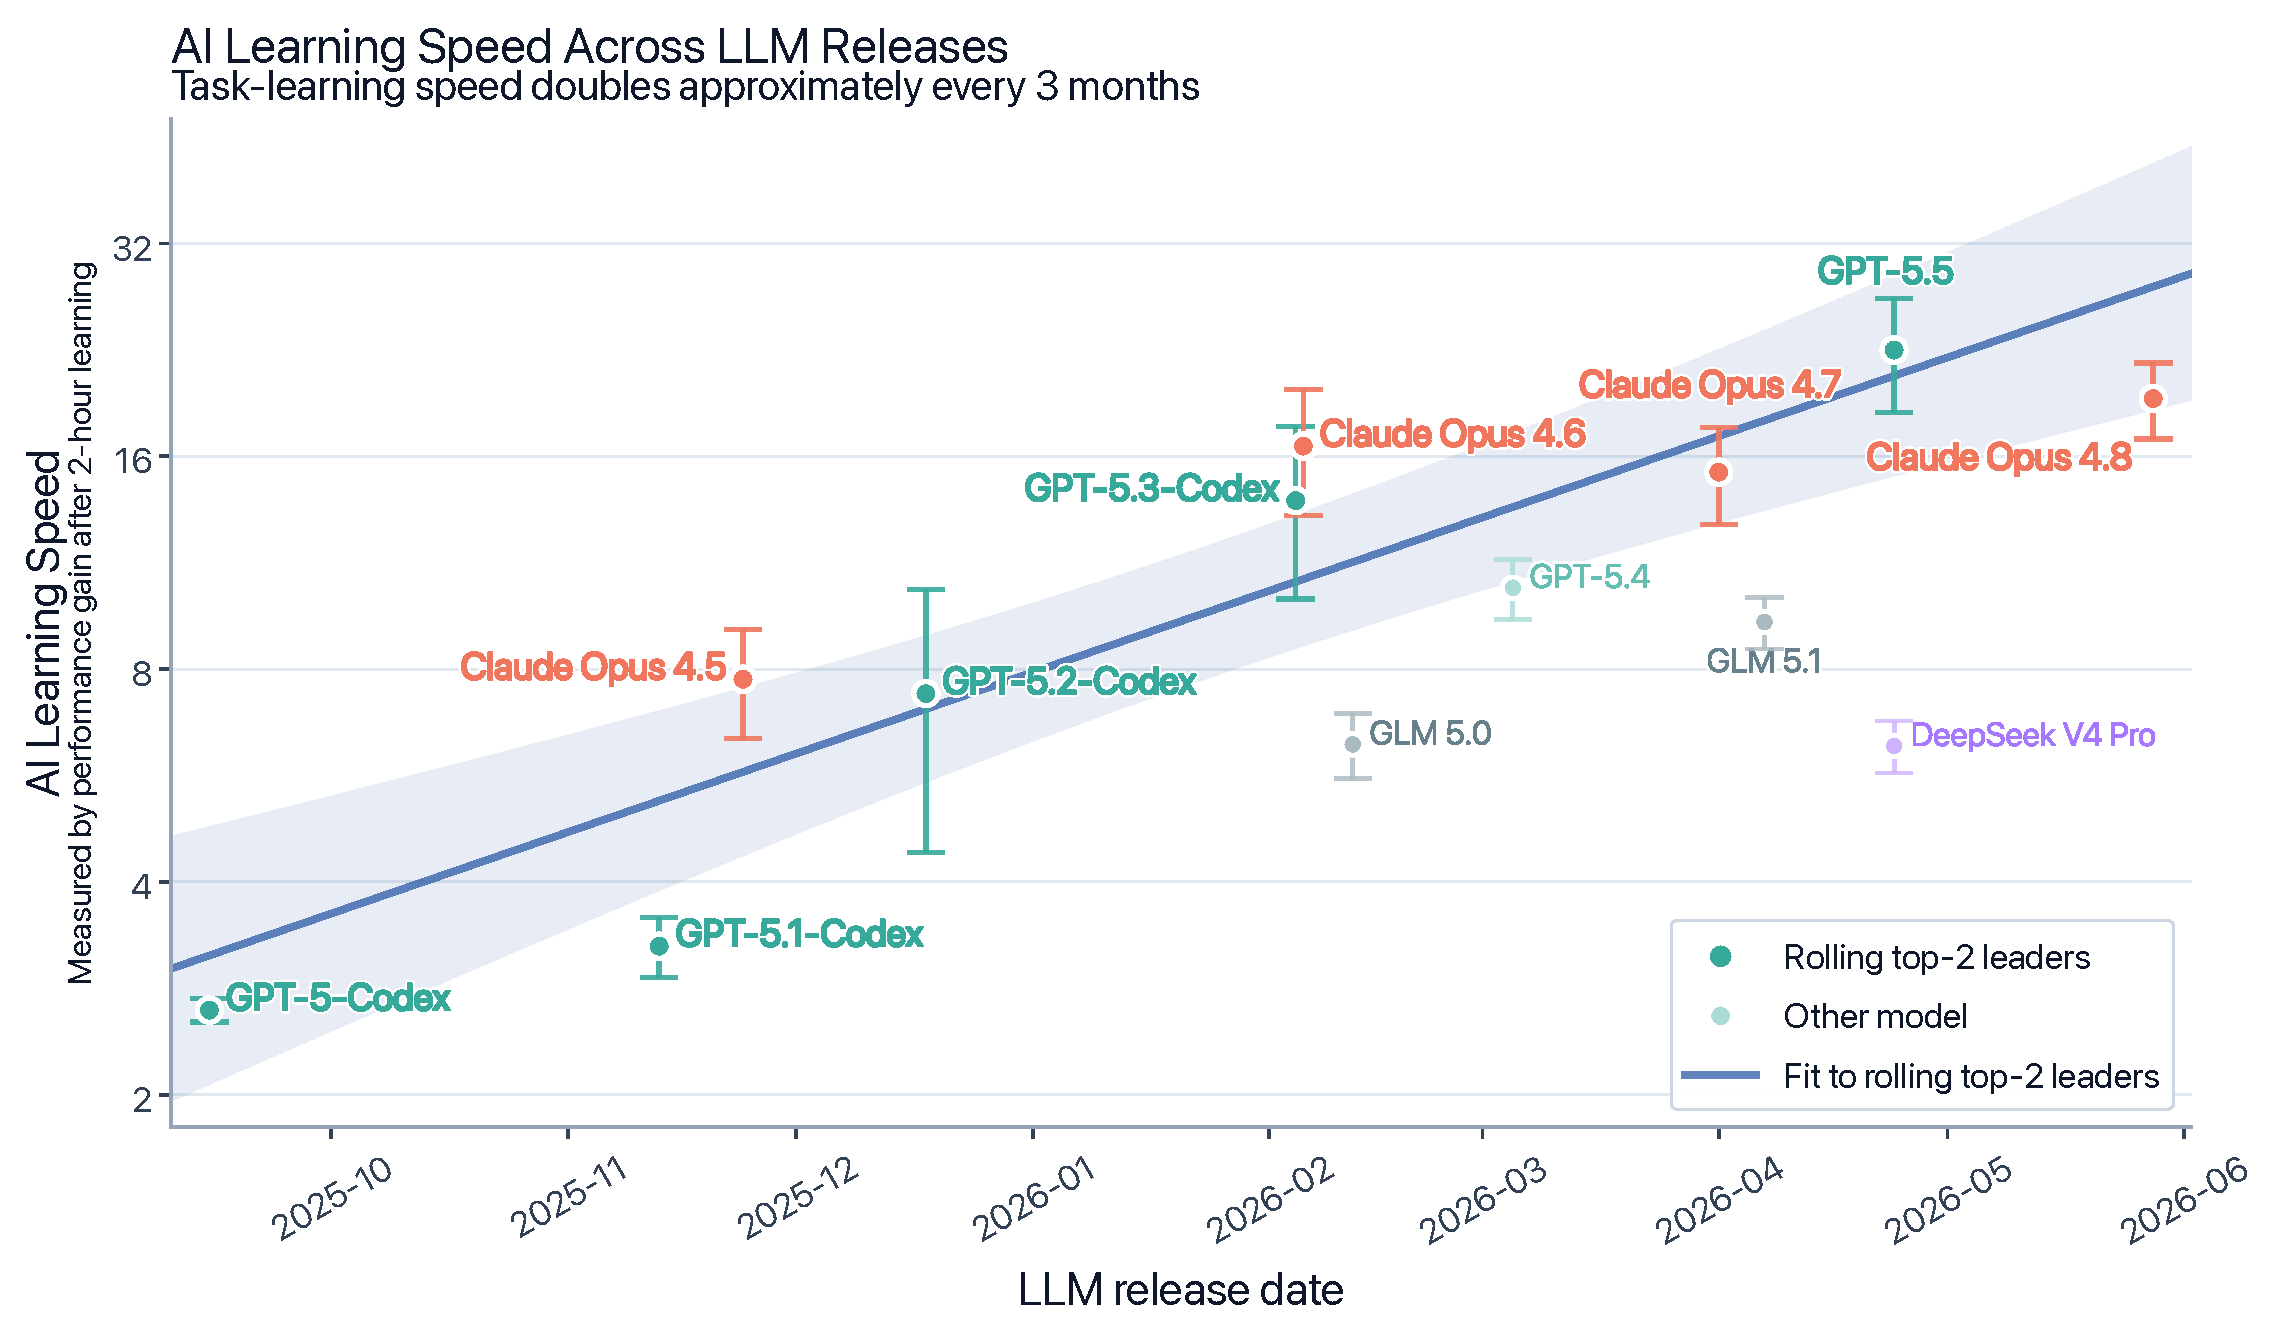
\includegraphics[width=0.9\linewidth]{figures/time_area_log2_curve.pdf}
\caption{Learning speed across evaluated LLM releases. Learning speed denotes the two-hour performance gain on the fixed 18-task slice. The blue line fits the rolling top-2 leaders by release date and indicates an approximately three-month doubling trend.}
\label{fig:scaling}
\end{figure}
